\section{Results and Analysis}\label{sec:results}

\subsection{Detection on MIO-TCD}\label{sec:results-detection}

Table~\ref{tab:det-test} reports the frozen test set. Fine-tuning raises
mAP@0.5 from 0.430 to 0.709 (MIO-only) and 0.720 (joint). The paired gains over
the pretrained detector are 0.279 and 0.291, with intervals that exclude zero.
No clear difference was established between the joint and MIO-only models on
this dataset (paired difference 0.011, 95\% CI −0.024 to 0.048). Counting error
roughly halves.
Figure~\ref{fig:detection-classes} gives the per-class breakdown.

\begin{table}[htbp]
  \centering
  \small
  \caption{Frozen MIO-TCD test set (2,000 images, human labels). mAP@0.5
  includes 95\% scene-group bootstrap intervals; other columns are point
  estimates.}
  \label{tab:det-test}
  \setlength{\tabcolsep}{3pt}
  \begin{tabular}{@{}lccccccc@{}}
    \toprule
    Model & mAP@0.5 & mAP@.5--.95 & Car & Moto. & Bus & Truck & Count MAE \\
    \midrule
    Pretrained YOLO26m & 0.429 (0.337--0.516) & 0.320 & 0.655 & 0.136 & 0.673 & 0.253 & 1.215 \\
    MIO-TCD only       & 0.709 (0.626--0.817) & 0.561 & \textbf{0.883} & 0.570 & \textbf{0.920} & \textbf{0.463} & \textbf{0.650} \\
    \rowcolor{oursrow}
    Joint fine-tuning  & \textbf{0.720} (0.645--0.825) & \textbf{0.563} & 0.874 & \textbf{0.646} & 0.908 & 0.453 & 0.698 \\
    \bottomrule
  \end{tabular}
  \par\smallskip
  \begin{minipage}{\linewidth}\footnotesize
    \textit{Note.} Bold marks the best value in each column; the shaded row is
    the joint model. The test set contains 33 motorcycle boxes; the motorcycle
    diagnostic split provides a larger sample.
  \end{minipage}
\end{table}

\begin{figure}[htbp]
  \centering
  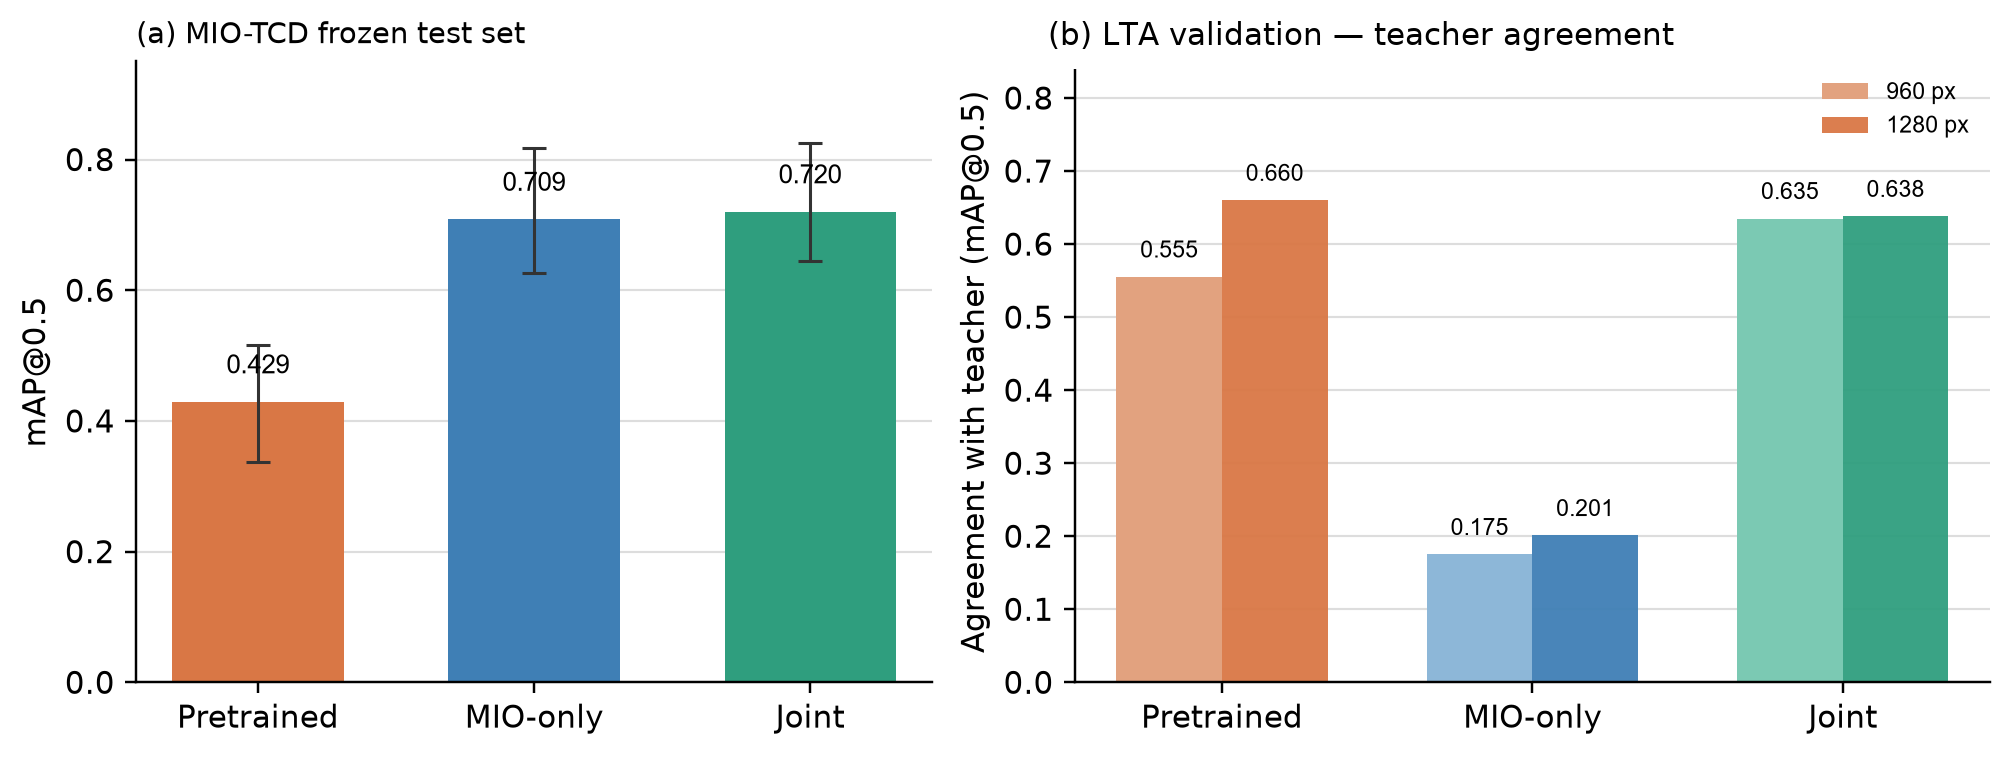
\includegraphics[width=0.96\linewidth]{detection_overall.png}
  \caption{Detection results. (a) Human-labeled MIO-TCD test set;
  (b) agreement with the YOLO26x teacher on LTA validation. The joint model is
  shown in green.}
  \label{fig:detection}
\end{figure}

\begin{figure}[htbp]
  \centering
  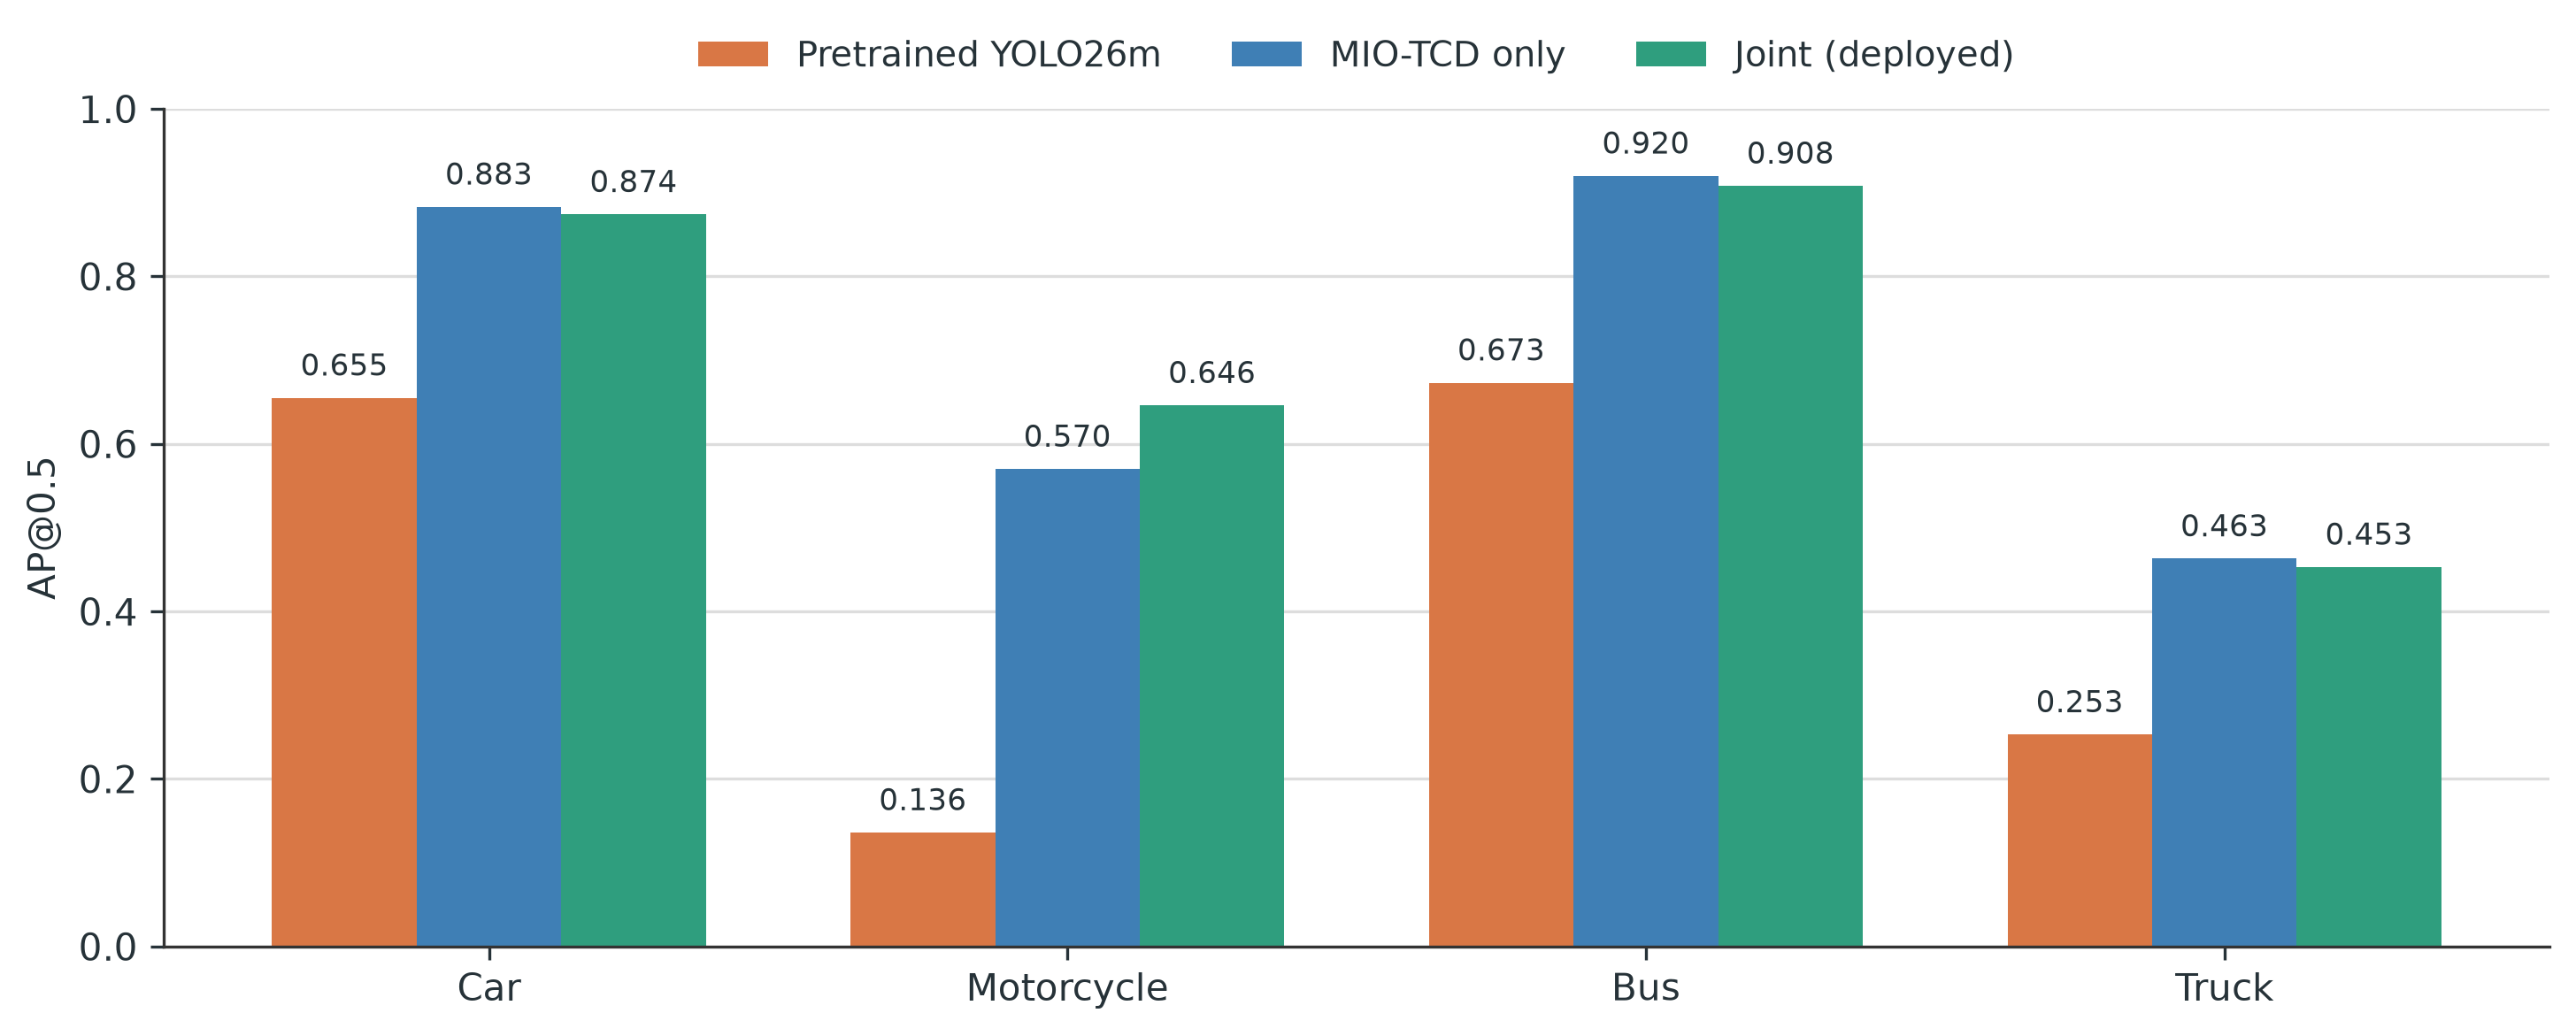
\includegraphics[width=0.96\linewidth]{detection_per_class.png}
  \caption{Per-class AP@0.5 on the frozen MIO-TCD test set. The joint model is
  shown in green and gives the largest gain on motorcycles.}
  \label{fig:detection-classes}
\end{figure}

\subsection{Cross-Domain Behavior on LTA}\label{sec:results-lta}

The LTA validation set uses the frozen YOLO26x pseudo-labels as its reference,
so the figures measure agreement with the teacher. The validation is evaluated
at 960 and 1280 pixels: 960 pixels is the lower-resolution setting used during
target-domain development, and 1280 pixels is the batch-inference resolution. At 960
pixels the pretrained model reaches 0.555, the MIO-only model 0.175, and the
joint model 0.635. The MIO-only result reflects the domain gap between North
American close-range views and the Singapore viewpoint.

At 1280 pixels, the batch-inference resolution, the pretrained model reaches
0.660 and the joint model 0.638. Agreement improves substantially over MIO-only
training, and the joint model's agreement is close to that of the pretrained
model at this resolution. The teacher row is a re-evaluation of YOLO26x at the
same inference resolutions after its labels were generated at 1920 pixels; it is
a reference point, not a mathematical upper bound on student performance.
Nighttime frames are the least reliable part of this proxy: low light and small
vehicle scale make both detection and manual annotation difficult. The
comparison is therefore a cross-domain proxy; accuracy across Singapore
traffic-camera conditions requires a human-labeled test set.
Figure~\ref{fig:model-comparison} gives a visual comparison on one frame. On
MIO-TCD the ranking reverses: MIO-only training reaches 0.709 mAP@0.5, compared
with 0.429 for the pretrained detector (Table~\ref{tab:det-test}). The joint
model is the compromise between the two domains.

\begin{table}[htbp]
  \centering
  \small
  \caption{LTA validation agreement with the frozen YOLO26x teacher (80 images,
  week~2).}
  \label{tab:lta}
  \begin{tabular}{@{}lccc@{}}
    \toprule
    Model & mAP@0.5 @960 & mAP@0.5 @1280 & Moto. AP@.5 @960 \\
    \midrule
    Pretrained YOLO26m & 0.555 & \textbf{0.660} & 0.539 \\
    MIO-TCD only       & 0.175 & 0.201 & 0.194 \\
    \rowcolor{oursrow}
    Joint fine-tuning  & \textbf{0.635} & 0.638 & \textbf{0.670} \\
    Teacher YOLO26x (re-evaluated) & 0.707 & 0.775 & 0.714 \\
    \bottomrule
  \end{tabular}
  \par\smallskip
  \begin{minipage}{\linewidth}\footnotesize
    \textit{Note.} Bold marks the best evaluated model in each column; the
    shaded row is the joint model. Teacher labels are model predictions. The
    teacher row re-evaluates YOLO26x at the same inference resolutions used for
    the students and serves as a reference, not an upper bound.
  \end{minipage}
\end{table}

\begin{figure}[H]
  \centering
  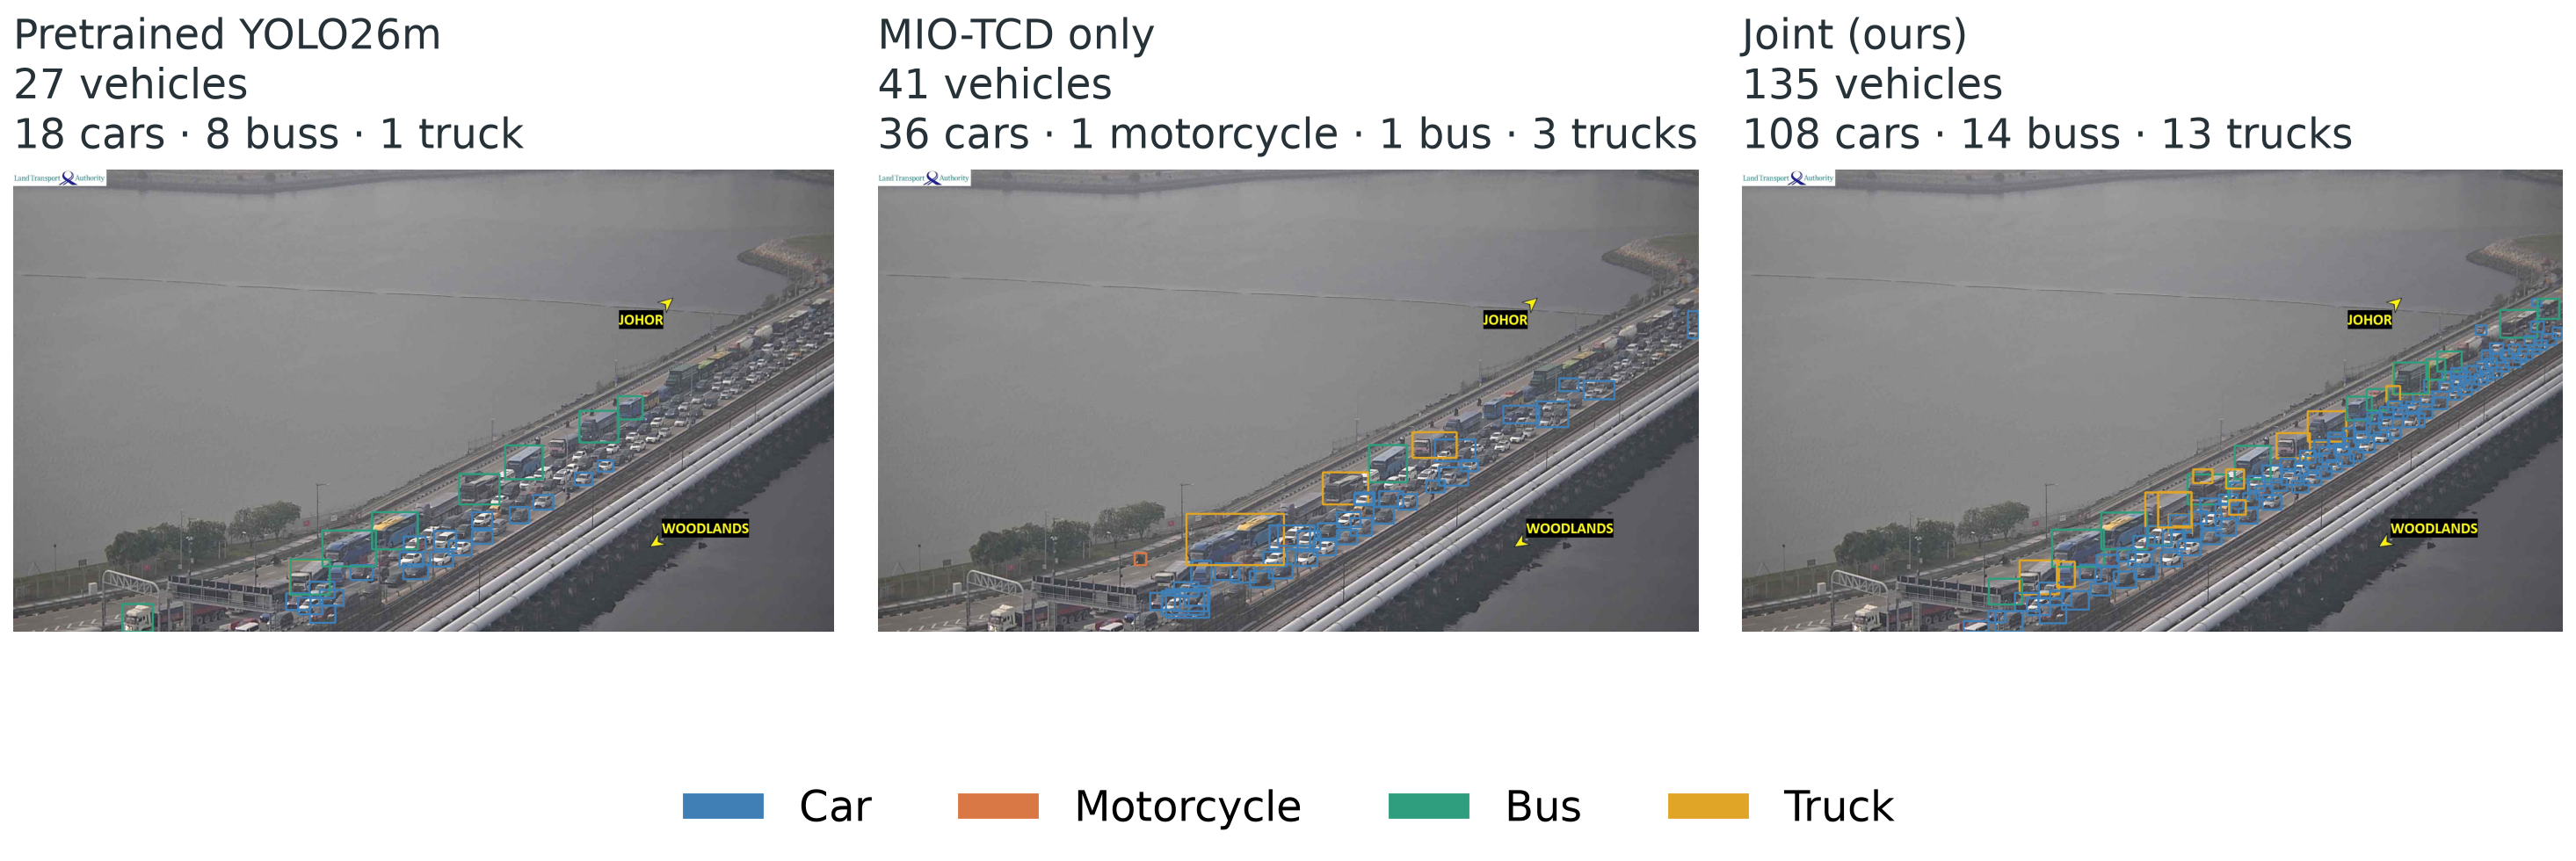
\includegraphics[width=\linewidth]{detection_model_comparison.png}
  \caption{Detection comparison on an LTA daytime frame (camera 2701, input
  1280, confidence 0.25). The pretrained detector finds 27 vehicles,
  MIO-TCD-only training 41, and joint fine-tuning 135. Box colors denote vehicle
  classes. The counts are model detections and illustrate detection density on
  one frame; they are not an accuracy measure. Table~\ref{tab:det-test} reports
  the quantitative comparison. On MIO-TCD the ranking reverses.}
  \label{fig:model-comparison}
\end{figure}

\subsection{Batch Inference on the LTA Collection}\label{sec:results-deployment}

The joint model was run over all 15,316 images at 1280 pixels with confidence
0.25. It produced 279,476 boxes: 187,928 cars, 41,109 motorcycles, 15,111 buses
and 35,328 trucks. The mean is 18.25 vehicles per frame, 27.22 during Singapore
daytime and 8.93 at night. A total of 1,478 frames returned zero detections,
1,437 of them at night. These frames are concentrated at night, where low light
and small vehicle scale limit both detection and manual verification. Nighttime
traffic volumes are also lower, so a zero-detection frame does not by itself
prove that vehicles were missed. The count is a detection count and may
understate nighttime traffic; the workbench's monitoring view presents it
alongside camera reliability indicators.

\subsection{Workbench}\label{sec:results-workbench}

The workbench presents the batch-inference outputs through three views. The
Overview view reports eight cameras, 15,316 processed frames, 279,476 detections
and the forecasting engine used for the speed target, together with camera and
forecast health and a needs-attention queue. The Monitoring view exposes
per-camera reliability (zero-detection rate, completeness and mean confidence), a
time-controlled detection frame and per-class counts. The Forecast view provides
replay-time and 15/30/60-minute horizon controls, a predicted-severity network
schematic, an observed and forecast speed curve with an empirical residual band,
and the threshold-based risk ranking defined in
Section~\ref{sec:method-workbench}. The interface marks the historical replay
state, and each view labels its data source; the Forecast view identifies PEMSD8
as a public California road-network dataset separate from the LTA cameras. The
service layer performs consistency checks against the recorded metrics and
reports warnings when output sets are incomplete or inconsistent.

\subsection{Forecasting: Eight-Model Comparison}\label{sec:results-forecast}

Table~\ref{tab:forecast-default} reports the default-configuration comparison.
GWNET has the lowest MAE among the evaluated configurations (14.648), followed
by MultiHeadSTGCN (14.839), MTGNN (15.106) and AGCRN (15.612). The configurations differ in input channels and
training recipes, so the table compares complete methods under the repository's
public protocol. The graph column distinguishes models that use the fixed road
adjacency from those that learn a graph or node embeddings.

\begin{table}[htbp]
  \centering
  \small
  \caption{Eight-model forecasting comparison on PEMSD8 traffic flow, default
  configuration, seed~0.}
  \label{tab:forecast-default}
  \begin{tabular}{@{}llcccc@{}}
    \toprule
    Model & Graph & Input channels & MAE & RMSE & MAPE (\%) \\
    \midrule
    GWNET                & Learned graph & 1 & \textbf{14.648} & \textbf{23.504} & \textbf{9.78} \\
    MTGNN                & Learned graph & 2 & 15.106 & 23.756 & 10.53 \\
    \rowcolor{oursrow}
    MultiHeadSTGCN & Road adjacency & 9 & 14.839 & 23.614 & 9.91 \\
    AGCRN                & Learned embeddings & 1 & 15.612 & 24.474 & 10.31 \\
    STGCN                & Road adjacency & 1 & 17.436 & 26.577 & 10.96 \\
    GRU                  & None & 2 & 19.706 & 32.363 & 12.27 \\
    FNN                  & None & 1 & 21.246 & 32.461 & 13.30 \\
    LSTM                 & None & 2 & 21.779 & 36.121 & 13.24 \\
    \bottomrule
  \end{tabular}
  \par\smallskip
  \begin{minipage}{\linewidth}\footnotesize
    \textit{Note.} Bold marks the lowest error in each column; the shaded row is
    the project's model. Road adjacency is the symmetrized PEMSD8 sensor-link
    graph; learned graphs and embeddings are estimated from data. Native input
    channels: 1 = flow; 2 = flow + time-of-day; 9 = flow + time-of-day + seven
    day-of-week one-hot features. MAE is in vehicles per five-minute interval.
    Default configurations also differ in training settings; this is a
    complete-method comparison.
  \end{minipage}
\end{table}

\subsection{The Custom Model: Ablation and Comparison}\label{sec:results-custom}

MultiHeadSTGCN is built on STGCN and keeps its temporal and spatial blocks. The
ablation ladder changes one design choice at a time within the custom
implementation, but the reference STGCN is the LibCity implementation. The two
also differ in training loss (masked MSE for STGCN, masked MAE for the custom
model), input features and multi-step strategy. The ladder therefore measures
the combined effect of the listed choices, not an isolated architecture effect.

Direct multi-step output lowers MAE from 17.61 to 16.05 (8.9\%). Adding
time-of-day and day-of-week lowers it to 15.00, an additional 6.5\% and a
cumulative 14.8\% relative to 17.61; day-of-week alone has little effect, while
the combination with time-of-day is stronger than either feature alone.
Chebyshev convolution on the symmetrized road adjacency lowers MAE to 14.90
(0.7\%); this difference is close to the 0.5\% variability observed when the same
configuration is rerun, so it is an observation rather than a stable gain. The
directed dual-path variant gives 14.91. Figure~\ref{fig:ablation} summarizes the
ladder.

Three comparisons should be kept separate. In the default-configuration
benchmark, STGCN (17.44) and MultiHeadSTGCN (14.84) differ by 14.9\%. In the
unified nine-channel benchmark, STGCN (16.11) and MultiHeadSTGCN (14.84) differ
by 7.9\%. The staged ablation above uses a different STGCN reference (17.61).
These are complete-recipe comparisons and are not interchangeable.

\begin{figure}[htbp]
  \centering
  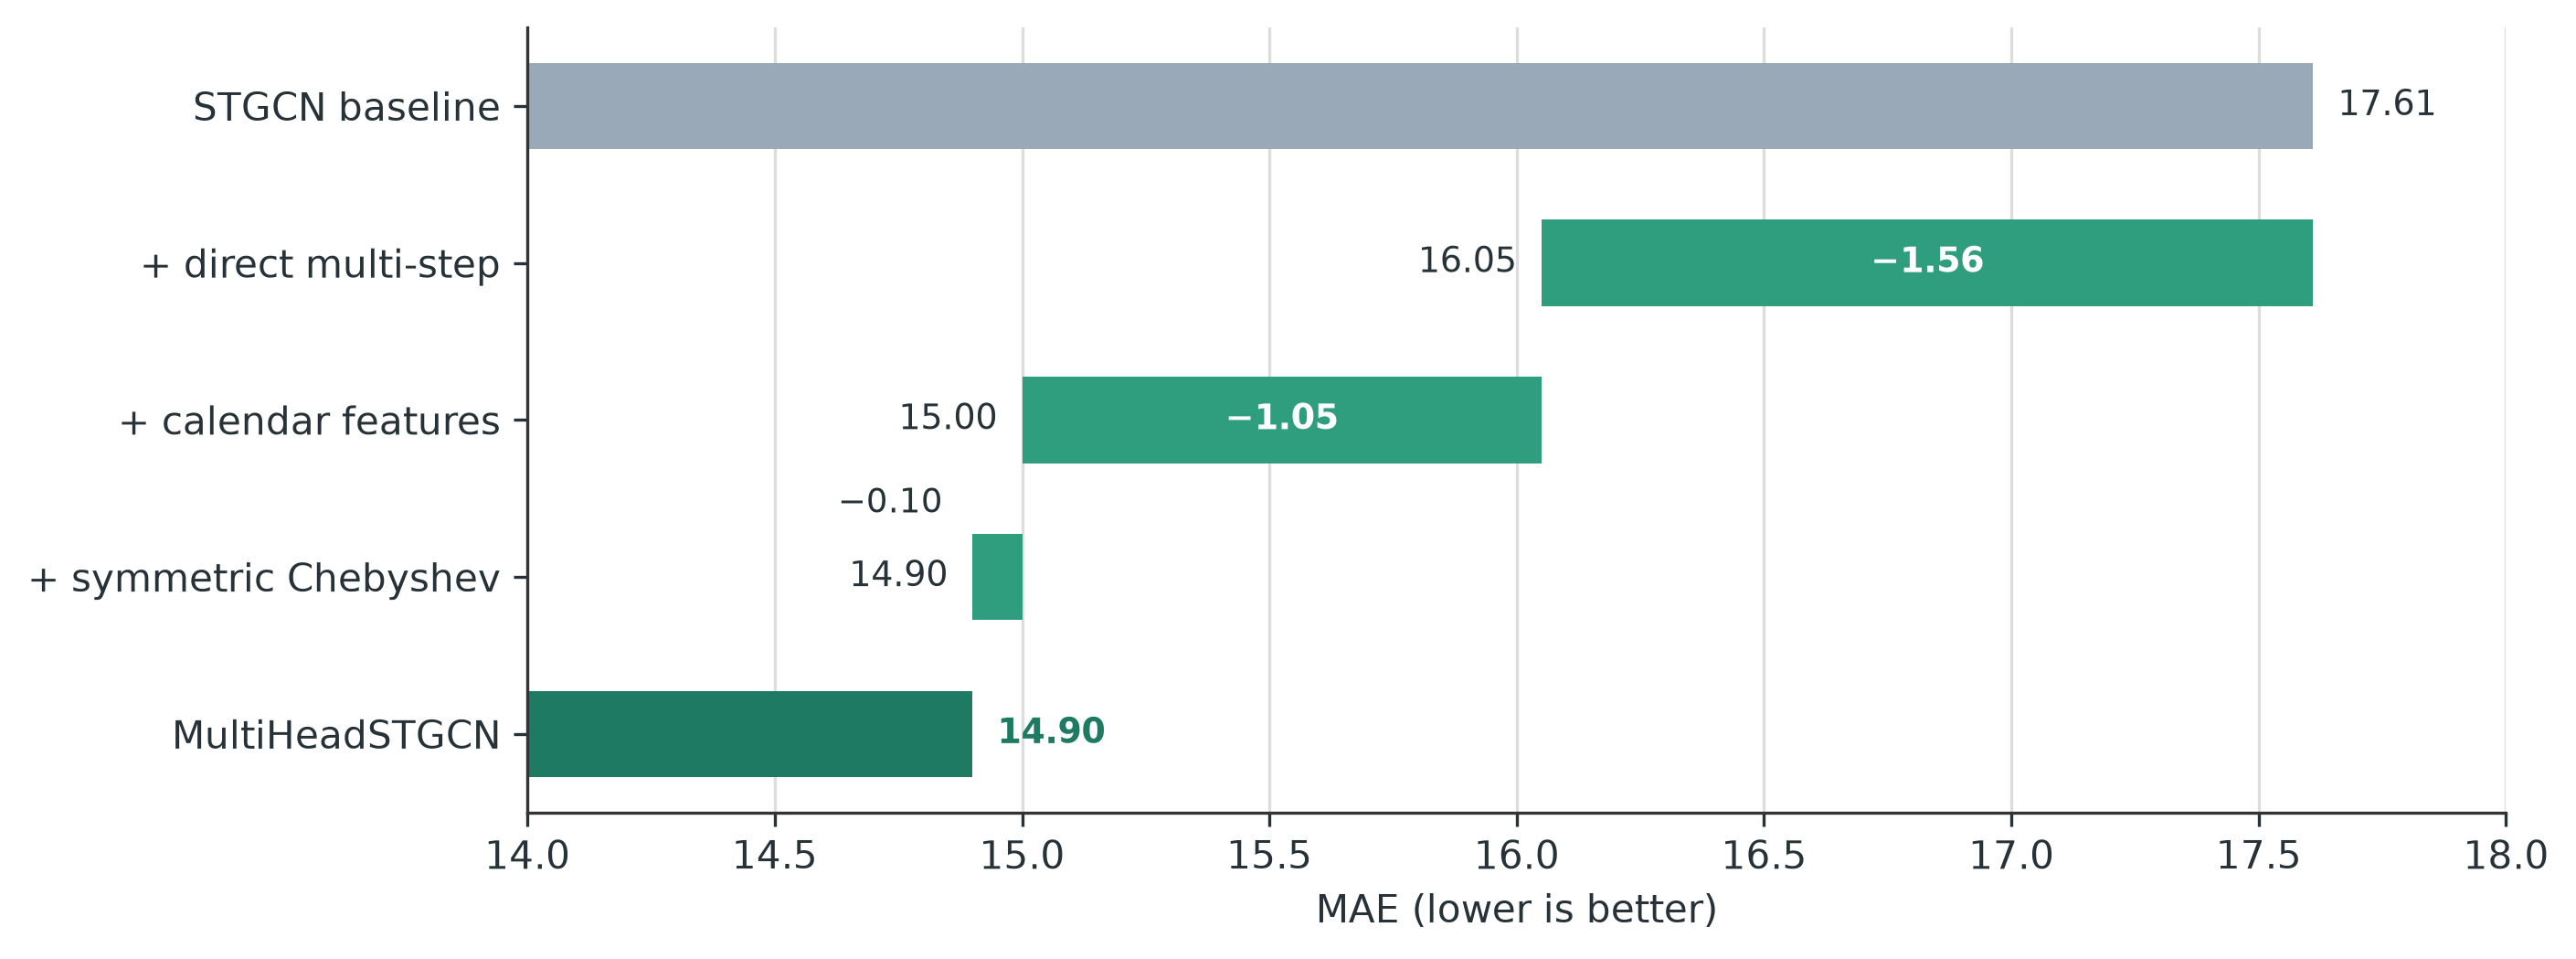
\includegraphics[width=0.9\linewidth]{forecast_ablation.png}
  \caption{Ablation of MultiHeadSTGCN on PEMSD8 traffic flow. Bars show
  absolute MAE; labels give the change from the preceding configuration. The
  x-axis starts at 14 to make the differences visible.}
  \label{fig:ablation}
\end{figure}

In the default-configuration table, MAE is 17.44 for STGCN and 14.84 for
MultiHeadSTGCN, a 14.9\% difference between complete recipes. Under default
configurations the model ranks second, after GWNET (14.648) and ahead of MTGNN
(15.106) and AGCRN (15.612). Under the unified nine-channel input it ranks fourth, after GWNET
(14.365), MTGNN (14.713) and AGCRN (14.777). With five seeds, GWNET's advantage
is 4.22\% (14.1995 versus 14.8256); the paired differences for MTGNN (14.7443)
and AGCRN (14.8913) have confidence intervals that include zero.

\subsection{Unified Input and Multi-Seed Check}\label{sec:results-seeds}

Table~\ref{tab:forecast-unified} reports the unified nine-channel setting. At
seed~0, GWNET is first (14.365), followed by MTGNN (14.713), AGCRN (14.777) and
MultiHeadSTGCN (14.839). The top four were selected by seed-0 test MAE and
re-run with seeds 0--4; this selection is exploratory, and the five-seed
comparison is descriptive rather than a pre-registered confirmatory test. Their
means and paired differences are reported in the same table. GWNET's paired advantage
over MultiHeadSTGCN is −4.22\% (95\% CI −4.98\% to −3.47\%, better on 5/5
seeds). The paired confidence intervals for MTGNN (−0.55\%, CI −1.29\% to
+0.20\%) and AGCRN (+0.44\%, CI −0.38\% to +1.27\%) include zero. Across five
paired seeds, no clear performance difference was established between
MultiHeadSTGCN and MTGNN or AGCRN. These results suggest comparable observed MAE
values, but the limited number of seeds prevents a strong equivalence claim.
GWNET achieved the lowest mean MAE among the four models evaluated across five
seeds. MultiHeadSTGCN also has the smallest seed-to-seed standard deviation
(0.0429). Figure~\ref{fig:multiseed} shows the five-seed means and standard
deviations, and Table~\ref{tab:forecast-horizon} gives the corresponding
15/30/60-minute MAE.

\begin{table}[htbp]
  \centering
  \small
  \caption{Forecasting comparison with unified nine-channel input on PEMSD8
  traffic flow. Seed-0 values cover all eight models; mean ± SD and paired
  differences cover the top four over seeds 0--4.}
  \label{tab:forecast-unified}
  \begin{tabular}{@{}lccc@{}}
    \toprule
    Model & MAE (seed 0) & MAE mean ± SD (seeds 0--4) & \shortstack{Paired diff\\vs MultiHeadSTGCN} \\
    \midrule
    GWNET                & \textbf{14.365} & \textbf{14.1995 ± 0.1022} & −4.22\% ± 0.61\% \\
    MTGNN                & 14.713 & 14.7443 ± 0.0893 & −0.55\% ± 0.60\% \\
    \rowcolor{oursrow}
    MultiHeadSTGCN & 14.839 & 14.8256 ± 0.0429 & -- \\
    AGCRN                & 14.777 & 14.8913 ± 0.0773 & +0.44\% ± 0.67\% \\
    STGCN                & 16.108 & -- & -- \\
    GRU                  & 21.722 & -- & -- \\
    FNN                  & 18.721 & -- & -- \\
    LSTM                 & 25.782 & -- & -- \\
    \bottomrule
  \end{tabular}
  \par\smallskip
  \begin{minipage}{\linewidth}\footnotesize
    \textit{Note.} Bold marks the lowest MAE; the shaded row is the project's
    model. MAE is in vehicles per five-minute interval. All models use nine
    channels: flow, time-of-day (one normalized channel) and day-of-week (seven
    one-hot channels). Mean ± SD describes seed-to-seed variation; the paired
    differences and their 95\% intervals are separate statistics and should not
    be read as standard deviations. Five-seed statistics cover the top four
    only. Negative paired differences mean the baseline has lower MAE than
    MultiHeadSTGCN.
  \end{minipage}
\end{table}

\begin{table}[htbp]
  \centering
  \small
  \caption{MAE by forecast horizon under the unified nine-channel input, mean ±
  SD over seeds 0--4.}
  \label{tab:forecast-horizon}
  \begin{tabular}{@{}lcccc@{}}
    \toprule
    Model & 15 min & 30 min & 60 min & 12-step average \\
    \midrule
    GWNET          & \textbf{13.431 ± 0.084} & \textbf{14.219 ± 0.099} & \textbf{15.465 ± 0.154} & \textbf{14.199 ± 0.102} \\
    MTGNN          & 13.951 ± 0.090 & 14.731 ± 0.091 & 16.035 ± 0.108 & 14.744 ± 0.089 \\
    AGCRN          & 14.137 ± 0.067 & 14.893 ± 0.090 & 16.094 ± 0.121 & 14.891 ± 0.077 \\
    \rowcolor{oursrow}
    MultiHeadSTGCN & 14.233 ± 0.044 & 14.832 ± 0.045 & 15.924 ± 0.068 & 14.826 ± 0.043 \\
    \bottomrule
  \end{tabular}
  \par\smallskip
  \begin{minipage}{\linewidth}\footnotesize
    \textit{Note.} MAE is in vehicles per five-minute interval. The 15, 30 and
    60 minute horizons correspond to output steps 3, 6 and 12. Values are means
    over seeds 0--4; ± is one standard deviation across seeds, not a confidence
    interval.
  \end{minipage}
\end{table}

\begin{figure}[htbp]
  \centering
  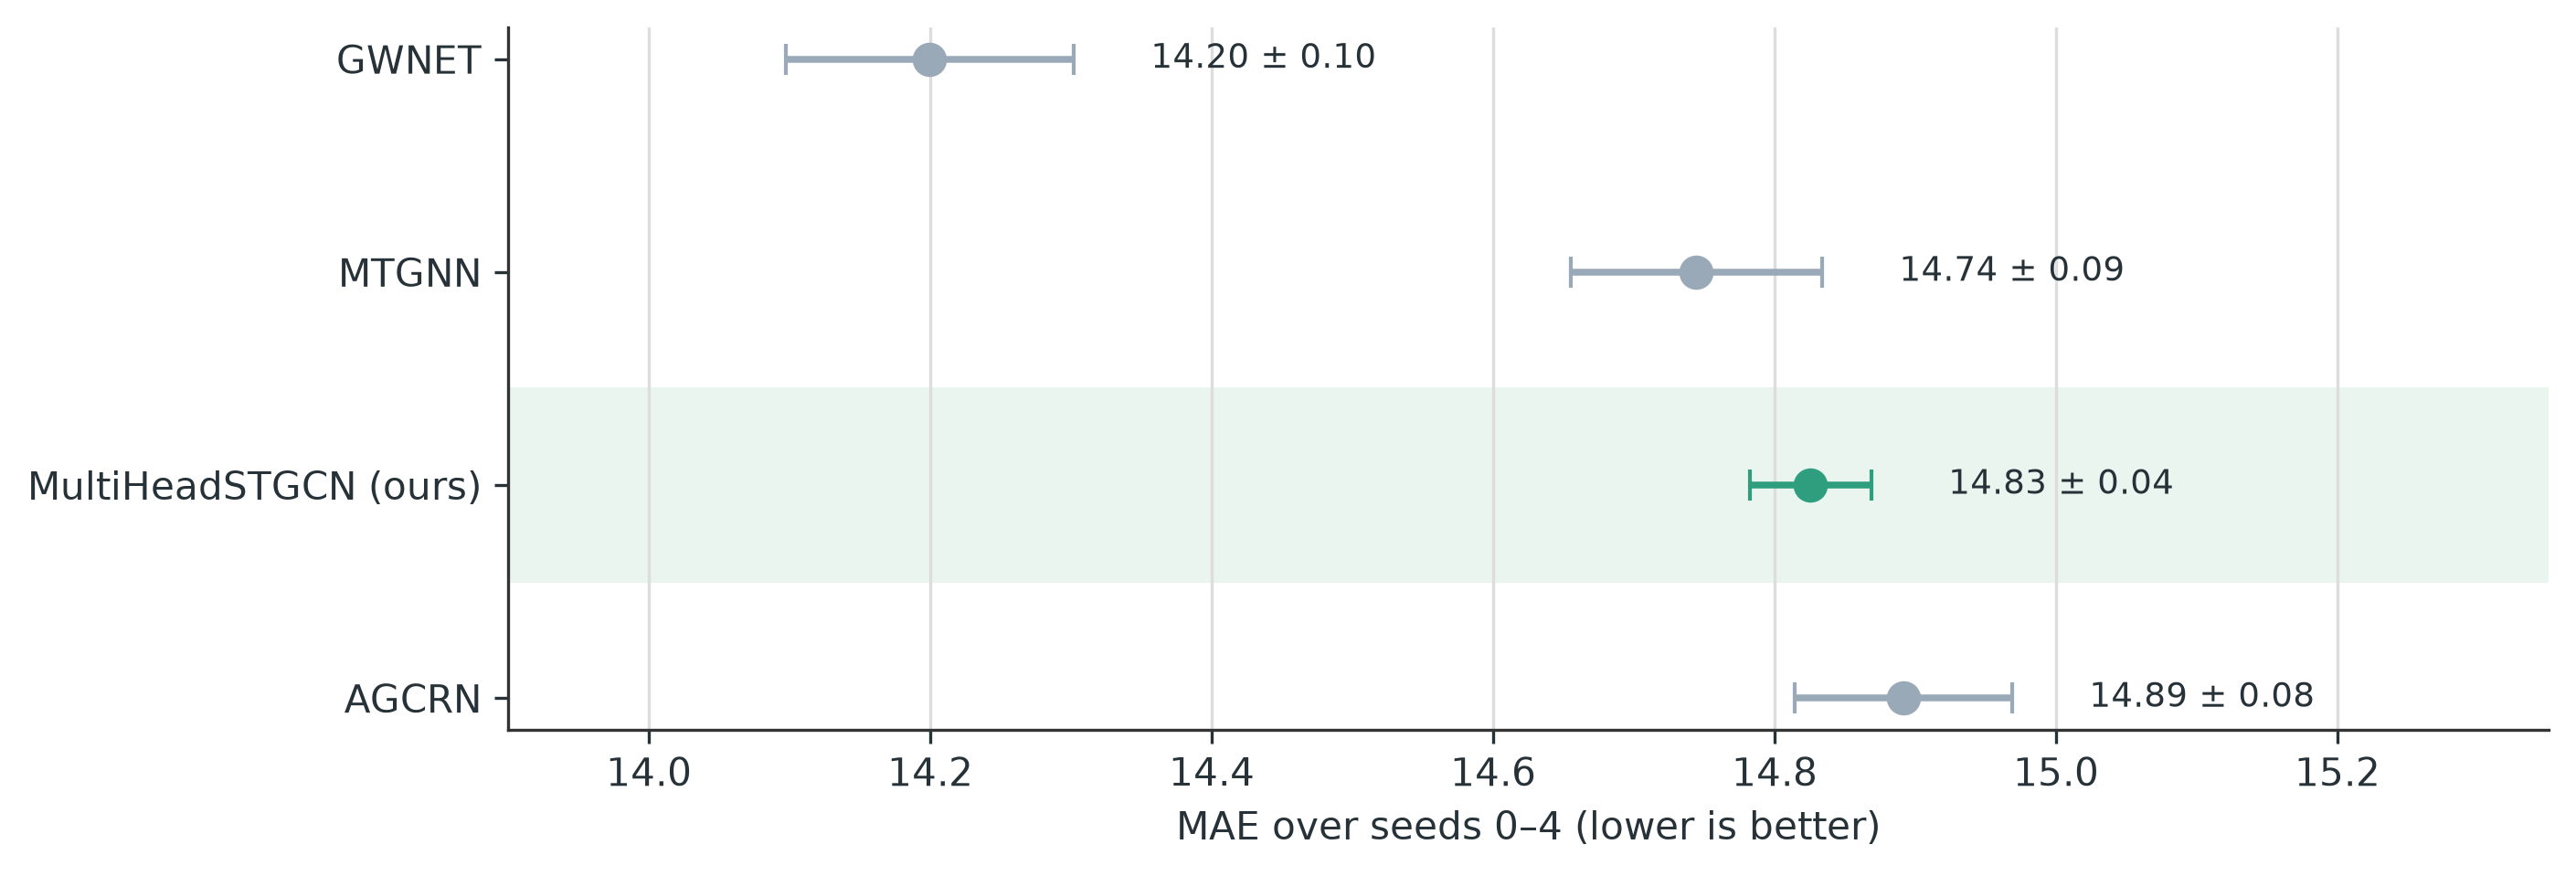
\includegraphics[width=0.9\linewidth]{forecast_multiseed.png}
  \caption{Five-seed MAE on PEMSD8 with unified nine-channel input. Points are
  means over seeds 0--4; error bars show ±1 SD and are not confidence
  intervals.}
  \label{fig:multiseed}
\end{figure}

\subsection{Ablation Findings}\label{sec:results-ablation}

Two ablations are reported. First, calendar features have model-dependent
effects. Adding time-of-day and day-of-week reduces MAE by 11.9\% for FNN,
7.6\% for STGCN, 5.3\% for AGCRN, 2.6\% for MTGNN and 1.9\% for GWNET, and
increases MAE by 10.2\% for GRU and 18.4\% for LSTM. LibCity's RNNs concatenate
all nodes and channels into one vector, so the nine-channel input becomes
1,530-dimensional and is harder to optimize with the default learning rate.

Second, a backbone-matched comparison examines the combined effect of the
changes. MultiHeadSTGCN reduces MAE from 17.61 (STGCN) to about 15.00 (14.8\%),
but because the loss, input features and multi-step strategy also differ, the
reduction cannot be attributed to architecture alone. Multi-target training was
also evaluated; the multi-target variant, which is the only setting that
exercises multiple heads, did not improve flow over the single-target
configuration, so the benchmark uses one target head.

% HUMAN-LTA-SLOT:
% When the human-labeled LTA test set is frozen and evaluated, insert
%     % Human-labeled LTA evaluation.
%
% This file is not included in main.tex yet. To enable it:
%   1. Freeze the human-labeled LTA test set and run the same evaluator used
%      for the teacher-reference results.
%   2. Replace the placeholders below with the new sample size, metrics and
%      interpretation.
%   3. Add % Human-labeled LTA evaluation.
%
% This file is not included in main.tex yet. To enable it:
%   1. Freeze the human-labeled LTA test set and run the same evaluator used
%      for the teacher-reference results.
%   2. Replace the placeholders below with the new sample size, metrics and
%      interpretation.
%   3. Add % Human-labeled LTA evaluation.
%
% This file is not included in main.tex yet. To enable it:
%   1. Freeze the human-labeled LTA test set and run the same evaluator used
%      for the teacher-reference results.
%   2. Replace the placeholders below with the new sample size, metrics and
%      interpretation.
%   3. Add \input{chapters/05-human-lta} at HUMAN-LTA-SLOT in
%      chapters/05-results-and-analysis.tex.
%
% Inserting this file after Section 5.8 makes it Section 5.9. Existing results
% tables and figures keep their numbers; only later appendix numbering may move.

\subsection{Human-Labeled LTA Evaluation}\label{sec:results-human-lta}

The LTA results in Section~\ref{sec:results-lta} use the frozen YOLO26x teacher
as reference. The human-labeled test set provides an independent accuracy
measurement, with the same four-class evaluator and the same confidence
threshold. It contains [N] images from [cameras and period].

Table~\ref{tab:lta-human} reports the three models on this set.

\begin{table}[htbp]
  \centering
  \small
  \caption{Human-labeled LTA test set ([N] images). mAP@0.5 includes 95\%
  bootstrap intervals.}
  \label{tab:lta-human}
  \begin{tabular}{@{}lccccccc@{}}
    \toprule
    Model & mAP@0.5 & mAP@.5--.95 & Car & Moto. & Bus & Truck & Count MAE \\
    \midrule
    Pretrained YOLO26m & -- & -- & -- & -- & -- & -- & -- \\
    MIO-TCD only       & -- & -- & -- & -- & -- & -- & -- \\
    Joint fine-tuning  & -- & -- & -- & -- & -- & -- & -- \\
    \bottomrule
  \end{tabular}
\end{table}

[Replace this paragraph with the quantitative comparison, confidence intervals
and the effect of replacing the teacher reference. If the conclusion differs
from Section~\ref{sec:results-lta}, state the difference explicitly.]

% Optional figure slot:
% \begin{figure}[htbp]
%   \centering
%   \includegraphics[width=\linewidth]{human_lta_examples.png}
%   \caption{Detection examples on the human-labeled LTA test set.}
%   \label{fig:human-lta-examples}
% \end{figure}
 at HUMAN-LTA-SLOT in
%      chapters/05-results-and-analysis.tex.
%
% Inserting this file after Section 5.8 makes it Section 5.9. Existing results
% tables and figures keep their numbers; only later appendix numbering may move.

\subsection{Human-Labeled LTA Evaluation}\label{sec:results-human-lta}

The LTA results in Section~\ref{sec:results-lta} use the frozen YOLO26x teacher
as reference. The human-labeled test set provides an independent accuracy
measurement, with the same four-class evaluator and the same confidence
threshold. It contains [N] images from [cameras and period].

Table~\ref{tab:lta-human} reports the three models on this set.

\begin{table}[htbp]
  \centering
  \small
  \caption{Human-labeled LTA test set ([N] images). mAP@0.5 includes 95\%
  bootstrap intervals.}
  \label{tab:lta-human}
  \begin{tabular}{@{}lccccccc@{}}
    \toprule
    Model & mAP@0.5 & mAP@.5--.95 & Car & Moto. & Bus & Truck & Count MAE \\
    \midrule
    Pretrained YOLO26m & -- & -- & -- & -- & -- & -- & -- \\
    MIO-TCD only       & -- & -- & -- & -- & -- & -- & -- \\
    Joint fine-tuning  & -- & -- & -- & -- & -- & -- & -- \\
    \bottomrule
  \end{tabular}
\end{table}

[Replace this paragraph with the quantitative comparison, confidence intervals
and the effect of replacing the teacher reference. If the conclusion differs
from Section~\ref{sec:results-lta}, state the difference explicitly.]

% Optional figure slot:
% \begin{figure}[htbp]
%   \centering
%   \includegraphics[width=\linewidth]{human_lta_examples.png}
%   \caption{Detection examples on the human-labeled LTA test set.}
%   \label{fig:human-lta-examples}
% \end{figure}
 at HUMAN-LTA-SLOT in
%      chapters/05-results-and-analysis.tex.
%
% Inserting this file after Section 5.8 makes it Section 5.9. Existing results
% tables and figures keep their numbers; only later appendix numbering may move.

\subsection{Human-Labeled LTA Evaluation}\label{sec:results-human-lta}

The LTA results in Section~\ref{sec:results-lta} use the frozen YOLO26x teacher
as reference. The human-labeled test set provides an independent accuracy
measurement, with the same four-class evaluator and the same confidence
threshold. It contains [N] images from [cameras and period].

Table~\ref{tab:lta-human} reports the three models on this set.

\begin{table}[htbp]
  \centering
  \small
  \caption{Human-labeled LTA test set ([N] images). mAP@0.5 includes 95\%
  bootstrap intervals.}
  \label{tab:lta-human}
  \begin{tabular}{@{}lccccccc@{}}
    \toprule
    Model & mAP@0.5 & mAP@.5--.95 & Car & Moto. & Bus & Truck & Count MAE \\
    \midrule
    Pretrained YOLO26m & -- & -- & -- & -- & -- & -- & -- \\
    MIO-TCD only       & -- & -- & -- & -- & -- & -- & -- \\
    Joint fine-tuning  & -- & -- & -- & -- & -- & -- & -- \\
    \bottomrule
  \end{tabular}
\end{table}

[Replace this paragraph with the quantitative comparison, confidence intervals
and the effect of replacing the teacher reference. If the conclusion differs
from Section~\ref{sec:results-lta}, state the difference explicitly.]

% Optional figure slot:
% \begin{figure}[htbp]
%   \centering
%   \includegraphics[width=\linewidth]{human_lta_examples.png}
%   \caption{Detection examples on the human-labeled LTA test set.}
%   \label{fig:human-lta-examples}
% \end{figure}

% here. The template is a separate Section 5.9; existing results tables,
% figures and section numbers stay unchanged. Keep the teacher-reference results in 5.2 as
% a separate proxy unless the new labels are intended to replace them.
